\chapter{Background}
This chapter describes theoretic results that this thesis is based
on. Should the reader already be familiar with machine learning, and
in particular Gaussian Processes, this chapter can be safely skipped.

\section{Trajectory Data}
A \textit{trajectory} $\traj_{k}$ of can be seen as an ordered collection of
observations $(x^{(k)}_1, x^{(k)}_2, \dots, x^{(k)}_N)$.
The thesis project focuses on \textit{spatio-temporal}
trajectories, which mean that each observation in a trajectory has a position both in time
and in space. A trajectory has a \textit{length} and
a \textit{duration}, where the length of a trajectory is its number of
observations $\len(\traj_{k}) = N$, and the duration is the time from the first
observation to the last $\dur(\traj_{k}) = \text{time}(x^{(k)}_N) - \text{time}(x^{(k)}_1)$. 
These properties are in general not the same for different
trajectories, which makes is difficult to compare trajectories in a
meaningful way. In particular, having a different length complicates
things. If a set of trajectories all have the same length, they could
be viewed as vectors, with one observation per dimension, and compared
using Euclidian distance. But trajectories of different lengths do not
exist in the same vector space, so Euclidian distance fails and more
advanced similarity metrics have to be used.
An illustration of trajectories with different length can be seen in Figure~\ref{fig:trajectory-projection-problems}.
\begin{figure}
  \centering
  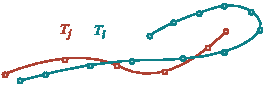
\includegraphics[width=0.7\textwidth]{figures/trajectory-projection-problems}
  \caption{An illustration of two trajectories $\traj_{i}$ and $\traj_{j}$
    with different lengths and duration. There is no natural way of
    measuring the distance between them.}\label{fig:trajectory-projection-problems}
\end{figure}

\section{Supervised Machine Learning}
Machine learning is the process of training computers programs to
recognise patterns in data~\ref{Bishop-2006}. It is incredibly
flexible, and can find patterns such as ``What
temperature is expected for this time of year on this geographical
position?'' or ``What subject is this text about?''. Finding the first
type of pattern of continuous temperature is called
\textit{regression}, and finding the
second pattern with a discrete number of subjects is called
\textit{classification}. Both types of problems have two inputs: 
the \textit{input matrix}
\[X =
  \begin{pmatrix}
    x_{1}^{1} & x_{2}^{1} & \cdots & x_{D}^{1} \\
    x_{1}^{2} & x_{2}^{2} & \cdots & x_{D}^{2} \\
    \vdots  & \vdots  & \ddots & \vdots  \\
    x_{1}^{N} & x_{2}^{N} & \cdots & x_{D}^{N} \\
  \end{pmatrix},
\]
containing $N$ samples, and the \textit{target vector} $Y = (y_{1},
y_{2}, \dots, y_{N})$. The
goal is to learn how the input and output is related by finding a model which approximates a $D$-ary function $y_n =
f(x_n)$ for $1 \leq n \leq N$. Such a model could then
\textit{predict} $y$ for a previously unseen input $\hat{x}$. However,
before predictions can be made, the model has to be \textit{trained}
on data. While there are many types of models, the remainder of this
section describes the process of training a model,
and using it to make predictions in a Bayesian framework.

\subsection{Model Training}
The first step is to pick a model for the data, which in a probabilistic
framework is a probability distribution $P(X \vert \theta)$, where
$\theta$ is a hyper-parameter vector to the probability distribution.
This is known as the \textit{likelihood}, which describes how likely
the data is given a certain $\theta$. One way of training a model is
by finding $\hat{\theta} = \underset{\theta}{\mathrm{argmax}} P(X \vert \theta)$, 
which is called \textit{maximum likelihood}-estimation (ML-estimation), since it picks the
$\theta$ that maximises the likelihood of the data. However, this picks a single
``best value'', highly sensitive to the choice of training data, which is sensitive to something called \textit{over-fitting}.

\begin{figure}
  \centering
  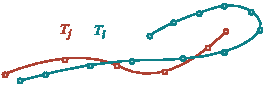
\includegraphics[width=0.7\textwidth]{figures/trajectory-projection-problems}
  \caption{TODO.}\label{fig:over-fitting-example}
\end{figure}

The goal when training a model is to learn patterns that
\textit{generalise} to unseen data, which typically mean that the
model can not be \textbf{too} flexible. Over-fitting is the phenomenon
when a model is too flexible and captures characteristics in data which could be
considered noise, which do \textbf{not} generalise. An example of
this can be seen in Figure~\ref{fig:over-fitting-example}. One way of
avoiding over-fitting is to use \textit{Bayesian inference}, in which 
Bayes theorem
\begin{equation}
  \label{eq:bayes}
  P(\theta \vert X) = \frac{P(X \vert \theta) P(\theta)}{P(X)}
\end{equation}
is used to estimate $\theta$ from the \textit{posterior} distribution $P(\theta \vert X)$.
This process is called \textit{maximum a posteriori}-estimation (MAP-estimation). To use Bayes
rule a \textit{prior} distribution $P(\theta)$ must be specified, which formalises
a prior belief about $\theta$ before observing any data. The prior is
subjective, and different people may pick different priors,
representing their personal belief in the data. By picking a
prior corresponding to a not-too-flexible model, over-fitting can be
avoided. In summary, the process of training a model is equivalent with computing
the posterior, from which the most probable model parameters can be
extracted.  

Training a model using ML- or MAP-estimation both require that the
likelihood can be optimised. This is not always possible to do in
closed form, in which case iterative methods, such as Stochastic
Gradient Descent (SGD) can be used. These types of methods are
prone to to finding local optimas, so random restarts need to be used
to increase the chances of finding a good parametrisation.

\subsection{Making Predictions}
When the model is trained, it can be used to make predictions
about new observations, via the \textit{posterior
  predictive distribution}
\begin{equation}
  \label{eq:posterior-predictive}
  P(y \vert X) = \int P(y|X,\theta)P(\theta \vert X) d \theta,
\end{equation}
which accounts for the parameter uncertainty through the
marginalisation of $\theta$. The resulting distribution over $y$ can
then be used to make predictions using a suitable statistic. 

\section{Arrival Time Prediction}
Arrival time prediction is, in a nutshell, the problem of answering
the question ``When does the bus arrive?''. Formally, the goal is to
learn a function $\arrtime = f(\obs)$ for arrival time $\arrtime$ and 
some vector $\obs$, which
contains information on the current state of the world. For instance, it
could contain the position of the closest vehicle and the time of day.

\subsection{Prediction Evaluation}
Two complementary ways of evaluating how good a prediction is are the metrics
\textit{Mean Absolute Error} (MAE) and \textit{Mean Absolute Percentage
  Error} (MAPE), defined for the true value $\hat{t}$ as 
\begin{equation}
  \label{eq:mae}
  MAE(\hat{t}, t) = \frac{1}{n}\sum_{i=1}^{n}{\vert \hat{t} - t \vert},
\end{equation}
and
\begin{equation}
  \label{eq:mape}
  MAPE(\hat{t}, t) = \frac{1}{n}\sum_{i=1}^{n} \vert \frac{\hat{t} - t}{\hat{t}} \vert
\end{equation}
respectively. 

Find source for criticism on MAPE. 
Find source for choosing MAE.

\section{Gaussian Processes}
A GP generalises a multivariate normal distribution, and can be seen
as a distribution over functions, completely defined by its
mean function $m(x)$ and covariance function, or kernel $k(x, x',
\theta)$~\cite{Rasmussen-Williams-2006}. Here, $x$ and $x'$ are
elements in the domain of modeled functions, and $\theta$ a
vector of hyper-parameters for the covariance function. For any input
vector $x$, the output $y$ is assumed jointly normally distributed according to
\begin{equation}
  \label{eq:gp}
  y = f(x) \sim \mathcal{N}(\mu(x), \Sigma(x))
\end{equation}
where
\begin{equation}
  \label{eq:gp-mean-function}
  \mu(x) = m(x) + K(x, \textbf{x})\textbf{V}^{-1}{(y-m(x))}^{T},
\end{equation}
\begin{equation}
  \label{eq:gp-covariance-function}
  \Sigma(x) = K(x, x) + \sigma^{2}_n\textbf{I} - \textbf{K}(x, \textbf{x})\textbf{V}^{-1}{\textbf{K}(x, \textbf{x})}^{T},
\end{equation}
and $\textbf{K}$ is the gram matrix with elements $K_{ij} = k(x_i, x_j)$ and $\textbf{V}
= K(x, x) + \sigma_n^2I$.
In the context of this thesis, the mean function $m(x)$ can be assumed to be $m(x) = 0$
without loss of generality, making the kernel $k(x, x', \theta)$
the only free parameter. Picking a specific kernel represents a prior
belief on how values close in $y$ are related, expressed in $x$. This
concept is explored in more detail in Section~\ref{sec:kernels-as-priors}.
Training a GP is typically done using maximum likelihood
estimation. That is, the GP parameters $\theta$ are optimised to
maximise the data likelihood. Unfortunately, this is non-convex
optimisation problem, so
iterative methods have to be used. The likelihood function is
non-convex, which introduces a high risk of finding local minimas
during the optimisation process. Because of this, random restarts are
typically required to find a good $\theta$.

\subsection{Kernel as Priors}\label{sec:kernels-as-priors}

Talk about different kernels and what prior beliefs they represent

\subsection{Gaussian Processes Regression}

\subsection{Structure Discovery Using Gaussian Processes}
